%\documentclass[11pt,twoside]{article}
\documentclass[11pt, french, A4wide]{article}
%\usepackage{makeidx}
\usepackage{index}
\usepackage[dvips]{graphicx}
\usepackage{color}
\usepackage{psfrag}
\usepackage{babel}
\usepackage{listings}
\usepackage{longtable}
\usepackage{mdwtab}
\usepackage{hhline}
\usepackage{amsmath}
\usepackage{amssymb}
\usepackage{amsthm}
\usepackage[latin1]{inputenc}
\usepackage[T1]{fontenc}
\usepackage{bbold}

\newlength{\malong}

\theoremstyle{remark}
\newtheorem{EXO}{Exercice}
\newenvironment{Exo}{\vspace{\parskip} \begin{EXO} \setlength{\malong}{\parskip}\setlength{\parskip}{0cm}$ $\par}
{\hspace*{\fill}$\triangle$\setlength{\parskip}{\malong}\end{EXO}}

\theoremstyle{definition}
\newtheorem*{COR}{Correction}
\newenvironment{Cor}{\vspace{\parskip} \begin{COR} \setlength{\malong}{\parskip}\setlength{\parskip}{0cm}$ $\par}
{\hspace*{\fill}$\blacktriangle$\setlength{\parskip}{\malong}\end{COR}}

\setlength{\oddsidemargin}{0cm}
\setlength{\evensidemargin}{0cm}
\setlength{\textwidth}{15.92cm}
\setlength{\textheight}{24cm}
\setlength{\footskip}{1.5cm}
\setlength{\topmargin}{-1cm}
\setlength{\headheight}{1cm}
\setlength{\headsep}{0.5cm}




\title{HPC and Uncertainty Treatment \\
 Examples with OpenTURNS and Uranie}
\author{EDF R\&D - PhiMeca - IMACS - CEA}
\date{Prace Advanced Training Center - 10-12 may 2021}


\begin{document}
  \maketitle


\vspace*{2cm}


\begin{minipage}{6cm}
  \begin{center}
    \begin{tabular}{c}
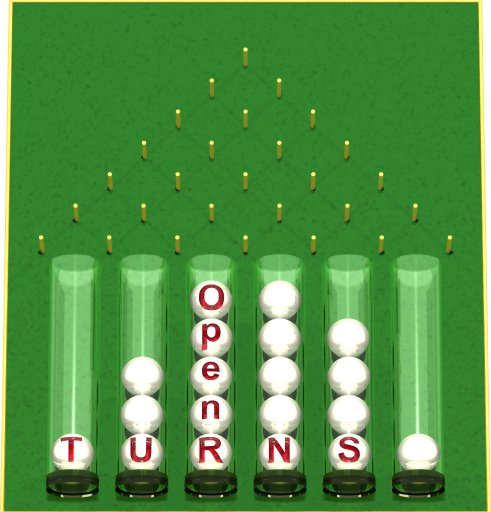
\includegraphics[height=5cm]{logoOpenTURNS.jpg}
    \end{tabular}
  \end{center}
\end{minipage}
\hfill
\begin{minipage}{6cm}
  \begin{center}
    \begin{tabular}{c}
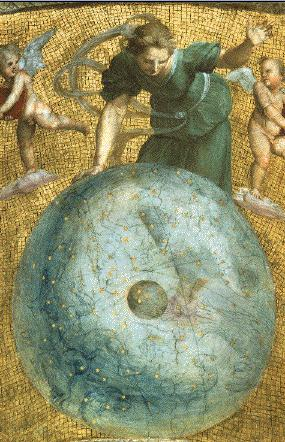
\includegraphics[height=5cm]{uranie_splash.png}
    \end{tabular}
  \end{center}
\end{minipage}

\vspace*{2cm}

\begin{minipage}{6cm}
%\begin{figure}[htbp]
  \begin{center}
    \begin{tabular}{c}
			
\includegraphics[width=5cm]{Prace_long.jpg}
    \end{tabular}
  \end{center}
%\end{figure}
\end{minipage}
\hfill
\begin{minipage}{6cm}
%\begin{figure}[htbp]
  \begin{center}
    \begin{tabular}{c}
				
\includegraphics[width=4cm]{logo_MDS.jpg}
    \end{tabular}
  \end{center}
%\end{figure}
\end{minipage}


\newpage
\section{Presentation of the study}

We study the deviation of a cantilever beam. An external force is applied to the free tip of the beam:

\begin{figure}[htbp]
\centering
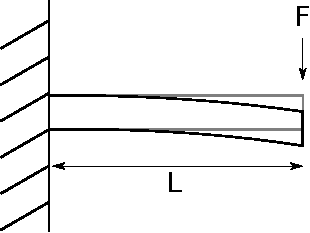
\includegraphics[width=4cm]{poutre.pdf}
\end{figure}

The vertical deviation writes:
\begin{equation}\label{relBeam}
  y = \displaystyle \frac{FL^3}{3EI}
\end{equation}
 where:
\begin{itemize}
    \item[$\bullet$]  E is the Young modulus,
    \item[$\bullet$]  F is the ponctual load,
    \item[$\bullet$]  L is the length of the beam,
    \item[$\bullet$]  I is the second moment of area according for bending.
\end{itemize}
\vspace*{0.2cm}

The ponctual values used for deterministic studies are:
$$
\left\{
\begin{array}{lcl}
 E & = & 3 \times 10^{9} \quad (Pa)\\
 F & = & 300  \quad (N)\\
 L & = & 2.5  \quad (m)\\
 I & = & 4 \times 10^{-6}  \quad (m^4)
\end{array}
\right.
$$
which correspond to $(3.0E7, 30000, 250, 400)$ when the length unit is the $cm$ rather than the $m$.\\

They correspond to the situation where a load of 30 kg is put at the extremity of a beam of length 2.5 m. It could be a diving platform in a swimming pool on which a 30kg-kid walks. \\

Uncertainties of the variables $(E,F,L,I)$ come from :
  \begin{itemize}
    \item[$\bullet$]  E : manufacturing defect of the material,
    \item[$\bullet$]  F : variation of the weight of the kid,
    \item[$\bullet$]  L :  manufacturing defect,
    \item[$\bullet$]  I :  manufacturing defect.
  \end{itemize}
\vspace*{0.2cm}

We observe a correlation between the uncertainties of the variables $L$ and $I$, due to the fabrication procedure of the beam: the greater $L$, the smaller $I$.


%%%%%%%%%%%%%%%
\newpage
\section{Uncertainty quantification}

We propose the following margins:

\begin{table}[h!]
	\begin{tabular}{|l|l|l|l|}
	\hline
	Variable & Description            & Distribution & Parameters and support                  \\ \hline
	E        & Young Modulus (Pa)     & from sample  & from sample (file \emph{sample\_E.csv}  \\ \hline
	F        & Load (N)               & Log-Normal   & $\mathbb{E}[F] = 30000$, $\sqrt{Var[F]} = 9000$, \\
             &                        &              & $[15000, +\infty[$   \\ \hline
	L        & Length (m)             & Uniform      & $[250; 260]$            				   \\ \hline
	I        & Bending moment ($m^4$) & Beta         & $r = 2.5,t = 4,a = 310,b = 450$         \\ \hline      
	\end{tabular}
\end{table}

\vspace*{0.2cm}

\begin{itemize}
 	\item Estimate the distribution of E from data by following methods:
  	\begin{enumerate}
		\item a parametric fitting with the Beta or Normal distribution. 
     	\item a non parametric fitting with the kernel smoothing method (normal kernel) or the histogram method.
   \end{enumerate}
   \item In both cases, the Kolmogorov validation test and QQ-Plot graph for each fitted distribution should be used to check the result. Then, plot the graph with the 3 ajusted densities (Beta, Normal and kernel smoothing) and compare them to each other.
\end{itemize}


\vspace*{0.2cm}

The dependence structure of the variables $(L,I)$ is the normal copula. We parameter the normal copula using the Spearman correlation $\rho_S<0$ which leads to the global Spearman correlation matrix:
$$
R_S = \left (
\begin{array}{cccc}
  1 & 0 & 0 & 0 \\
  0 & 1 & 0 & 0 \\
  0 & 0 & 1 & \rho_S \\
  0 & 0 & \rho_S & 1
\end{array}
\right)
$$
The Spearman correlation matrix has to be mapped into the normal correlation matrix.\\

Create the output random vector $Y$ defined by (\ref{relBeam}). Stay alert to the way gradients are evaluated.


%%%%%%%%%%%%%%%
\section{Central dispersion}

The objective of the study is to evaluate some central caracteristics of the distribution of Y as follows:
\begin{itemize}
 \item[$\bullet$] Estimate $\mathbb{E}(Y)$ using a Monte Carlo sampling: give the variance of the estimator and the confidence interval of level $95 \%$.
 \item[$\bullet$] Estimate $\mathbb{E}(Y)$ using the Taylor decomposition of $Y$ of order 1 and 2; give the importance factors of the input variables (stay alert to the correlated variables).
\end{itemize}
\vspace*{0.2cm}

To analyse the sensitivity of $Y$ to the input variables:
 \begin{itemize}
 \item[$\bullet$] Sample the input random vector and the output variable $Y$ and draw the clouds in the bivariate spaces  $(E,Y)$, $(F,Y)$, $(L,Y)$, $(I,Y)$.  Conclude.
 \item[$\bullet$] Estimate $\mathbb{E}(Y)$ using the Taylor decomposition of $Y$ of order 1 and 2; give the importance factors of the input variables.  Conclude.
 \item[$\bullet$] Draw the cobweb graph that links $Y$ and each input variable $E, F, L, I$. Conclude.
 \end{itemize}

\newpage
\section{Rare event probability}

We consider the event $Ev = \left\{Y(E,F,L,I) > s \right\}$, where $s = 30cm$.\\

Evaluate the probability $p=\mathbb{P}(E)$ using:
 \begin{itemize}
 \item[$\bullet$] the Monte Carlo estimator. Give the  confidence interval of level $95 \%$ of the estimator and draw the convergence graph.
 \item[$\bullet$] the FORM method and evaluate the global importance factors (stay alert to the correlated variables).
 \end{itemize}


\section{Metamodelling}

\subsection{Polynomial chaos approximation}

The objective is to approximate (\ref{relBeam}) with a chaos polynomial approximation, as follows: use the marginal polynomials which are orthogonal with respect to the marginal distributions, except for the LogNormal margin for which we use the Laguerre family.\\

Once the meta model is obtained:
\begin{itemize}
 \item[$\bullet$] evaluate the mean and the variance of the output random variable $Y$.
 \item[$\bullet$] evaluate the Sobol indices to analyse the sensitivity of $Y$ to different sets of the input variables.
 \item[$\bullet$] use this meta-model to re-evaluate $p=\mathbb{P}(E)$ using the Monte Carlo estimator. Conclude.
 \end{itemize}



\subsection{Kriging}

The objective is to approximate (\ref{relBeam}) with a kriging approach. Once the meta model is obtained, do the same actions as for the polynomial chaos approximation.



\end{document}
